\documentclass[a4paper, 12pt]{article}
\usepackage[russian]{babel}
\renewcommand{\baselinestretch}{1.5}
\usepackage[left=3cm,right=1.5cm,top=2cm,bottom=2cm]{geometry}
\setlength\parindent{1.25cm}
\usepackage{graphicx} %картинки
\usepackage{physics} %матрицы
\usepackage{multirow} %таблицы
\usepackage[x11names]{xcolor} %цвета
\usepackage{pgfplots} %графики
\pgfplotsset{compat=1.9} %версия pgfplots
\usepackage{float}
\usepackage{wrapfig} %рисунки сбоку
%\usepackage{gnuplottex} % Включаем Gnuplottex
\usepackage{array} % используется для установки фиксированной ширины столбцов
\usepackage{siunitx} % СИ

\usepackage{multicol}
\usepackage{lipsum}
\usepackage{mwe}

\usepackage{placeins}

\begin{document}

    % НАЧАЛО ТИТУЛЬНОГО ЛИСТА
    \begin{center}
        {Министерство науки и высшего образования Российской Федерации}\\
        {ФЕДЕРАЛЬНОЕ ГОСУДАРСТВЕННОЕ АВТОНОМНОЕ}\\ 
        {ОБРАЗОВАТЕЛЬНОЕ УЧРЕЖДЕНИЕ ВЫСШЕГО ОБРАЗОВАНИЯ}\\
        {«МОСКОВСКИЙ ФИЗИКО-ТЕХНИЧЕСКИЙ ИНСТИТУТ}\\
        {(НАЦИОНАЛЬНЫЙ ИССЛЕДОВАТЕЛЬСКИЙ УНИВЕРСИТЕТ)»}\\
        {(МФТИ, Физтех)}\\
    \end{center}
    
    \vspace{14em}
    
    \begin{center}
        {КАФЕДРА ОБЩЕЙ ФИЗИКИ}\\ %% ОБЩЕЙ ФИЗИКИ, ВАКУУМНОЙ ЭЛЕКТРОНИКИ 
        {ВОПРОС ПО ВЫБОРУ}\\
        {ИЗУЧЕНИЕ ДИФРАКЦИОННОЙ РЕШЁТКИ С ПОМОЩЬЮ САМОДЕЛЬНОГО СПЕКТРОСКОПА}\\
    \end{center}
    
    \vspace{15em} %16em когда название в 1 строку и один человек 12 электроника
    
    \normalsize
    { 
    \begin{tabular}{ m{5cm} m{1.5cm} l m{4cm} }
        Работу выполнил % & & \underline{\hspace{3.8cm}} & Я. А. Чемакина \\
        % & & \underline{\hspace{3.8cm}} & П. Ю. Шевелина \\
        & & \underline{\hspace{3.8cm}} & В. М. Шляпин \\
        & & \hspace{0.7632cm}\footnotesize{(подпись, дата)} & 
    \end{tabular}
    }

    \vspace{1em}

    \normalsize
    { 
    \begin{tabular}{ m{5cm} m{1.5cm} l }
        Работу принял, оценка & & \underline{\hspace{7.2cm}} \\
        & &\hspace{0.7632cm}\footnotesize{(подпись, дата, оценка)} 
    \end{tabular}
    }
    
    \vspace{3em} %3em когда название в 1 строку
    
    \begin{center}
        Москва, Долгопрудный 2025
    \end{center}

    \thispagestyle{empty} % выключаем отображение номера для этой страницы
	% КОНЕЦ ТИТУЛЬНОГО ЛИСТА

    \newpage
	
		\tableofcontents % Вывод содержания
	
	\newpage

	\section{Введение}
	
	\textbf{Цель работы:} собрать спектроскоп на основе дифракционной решётки 
	и найти период дифракционной решетки.\\
	\textbf{В работе используются:} 3 дифракционные решетки (500 штр/мм, 1000 штр/мм, двойная),
	веб-камера, лазерная указка с длиной волны 
	$\lambda = 405 \pm 10 \text{нм}$.
	
	\section{Теоретическая справка}

	\begin{multicols}{2}
        \begin{figure*}[ht!]
			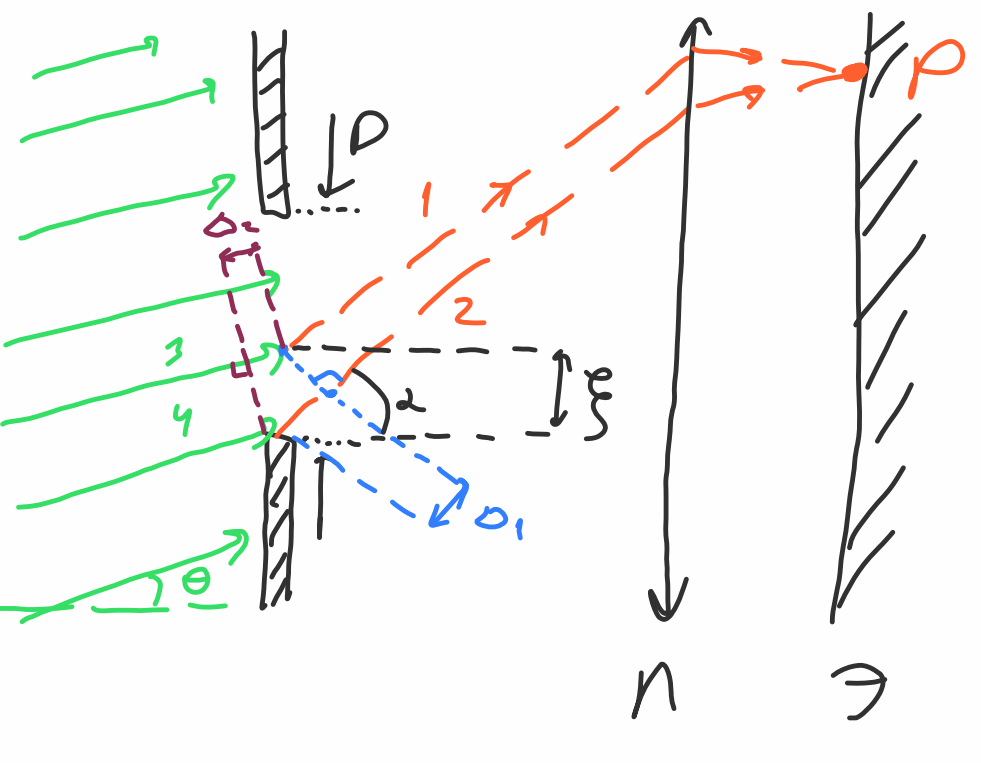
\includegraphics[width=8cm]{basa.png}\hfill
			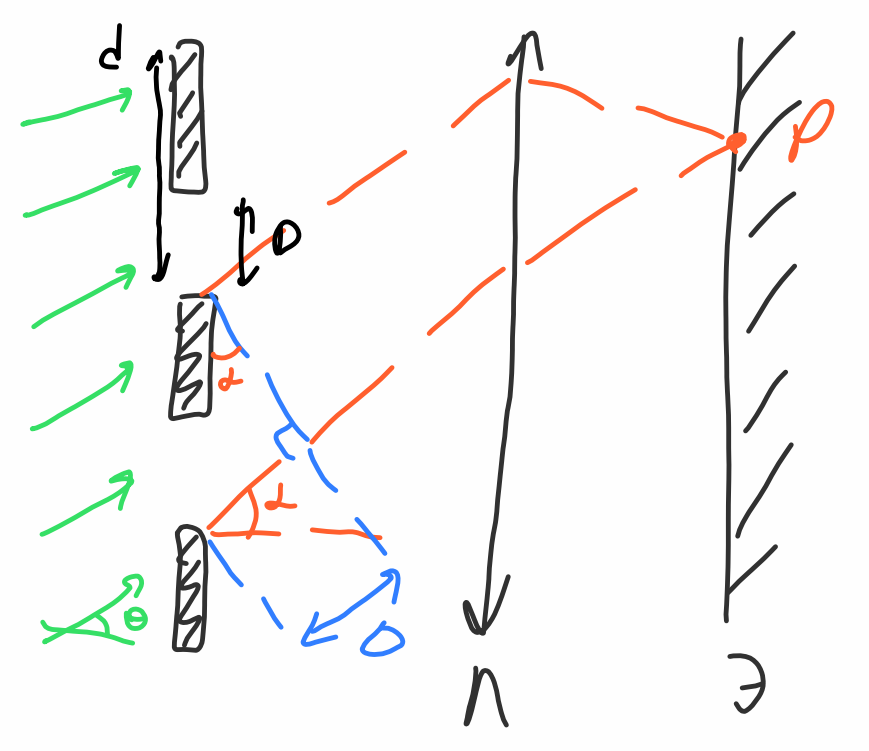
\includegraphics[width=8cm]{very_basa.png}\hfill
            \caption{Дифракция Фраунгофера на щели и дифракционная решетка}
			\label{fig: fig0}
        \end{figure*}
    \end{multicols}

	Сначала рассмотрим дифракцию Фраунгофера на щели (рис. \ref{fig: fig0}):
	$\Delta_1$ - разность хода между лучами 2 и 1, 
	$\Delta_2$ - разность хода между лучами 3 и 4. 
	$\Delta_1 = \xi sin(\alpha)$, $\Delta_2 = \xi sin(\theta)$. Тогда итоговая разность 
	хода $\Delta = \Delta_1 - \Delta_2 = \xi (sin(\alpha) - sin(\theta))$.
	Тогда вклад в амплитуду вектора напряженности от одного маленького кусочка: 
	$dA = A_0\cdot e^{ik\Delta}/D\cdot d\xi$

	Тогда запишем интеграл Френеля:
	$$f(p) = \frac{A_0}{D} \int_{-D/2}^{D/2} e^{ik\xi (sin(\alpha) - sin(\theta))} \,d\xi = 
	A_0\cdot\frac{sin(kD\cdot (sin(\alpha) - sin(\theta))/2)}
	{kD\cdot (sin(\alpha) - sin(\theta))/2}$$

	Теперь перейдем к решетке: $\Delta = d sin(\alpha)$ - разность хода между лучами из 
	двух щелей решетки. Тогда разность фаз: $\Delta \phi = k\Delta = 
	\frac{2\pi}{\lambda}d sin(\alpha)$. 
	От первой щели придет (в т. P) $E_1 = E_0\cdot\frac{sin(\gamma)}{\gamma}$, где 
	$\gamma = kD\cdot (sin(\alpha) - sin(\theta))/2$ из дифракции Фраунгофера. От второй щели 
	будет тоже самое, но сдвинутое по фазе на $\Delta \phi$, 
	$E_2 = E_1\cdot e^{-i\Delta \phi} = E_0\cdot\frac{sin(\gamma)}{\gamma}\cdot 
	e^{-i\Delta \phi}$ и так далее. Результурующую волну найдем как суперпозиция от всех волн, 
	т.е. от волн из всех щелей (N штук). Получим(сумма считается как геометрическая 
	прогрессия):
	$$E = \sum_{n = 1}^{N} E_n = E_1 \cdot \frac{1-e^{-iN\Delta \phi}}{1-e^{-i\Delta \phi}} = 
	E_1\cdot \frac{sin(N\Delta \phi/2)}{sin(\Delta \phi/2)} \cdot e^{-i(N-1)\Delta \phi}$$

	Тогда интенсивность: $I = I_1\cdot [\frac{sin(N\Delta \phi/2)}{sin(\Delta \phi/2)}]^2$, 
	где $I_1 = I_0\cdot [sin(\gamma)/\gamma]^2$. Тогда:

	$$I = I_0\cdot \Biggl[
	\frac{sin(kD\cdot (sin(\alpha) - sin(\theta))/2)}{kD\cdot (sin(\alpha) - sin(\theta))/2}
	\Biggr]^2\cdot\Biggl[\frac{sin(Nkdsin(\alpha)/2)}{sin(kdsin(\alpha)/2)}\Biggr]^2$$

	От сюда легко получить условие максимумов: 
	$kdsin(\alpha)/2 = \pi m$, или $dsin(\alpha) = \lambda m$. Также видно, что если 
	$sin(\alpha) = sin(\theta) $, то интенсивность будет максимальна. Тогда окончательно 
	можно получить что $dsin(\theta) = \lambda m$ условие максимума.


	\section{Ход работы}

	\subsection{Сборка спектроскопа}

	Сначала был собран сам спектрометр. Он состоит из основания с щелью, вращающегося 
	барабана, в котором закреплена камера и есть возможность устанавливать дифракционную решетку перед 
    камерой, а также крышки с закрепленным транспортиром транспортиром для измерения угла поворота барабана.

	Ниже представлены некоторые фото с процесса сборки и фото конечного вида спектроскопа. 

	\begin{figure}[H]
        \centering
        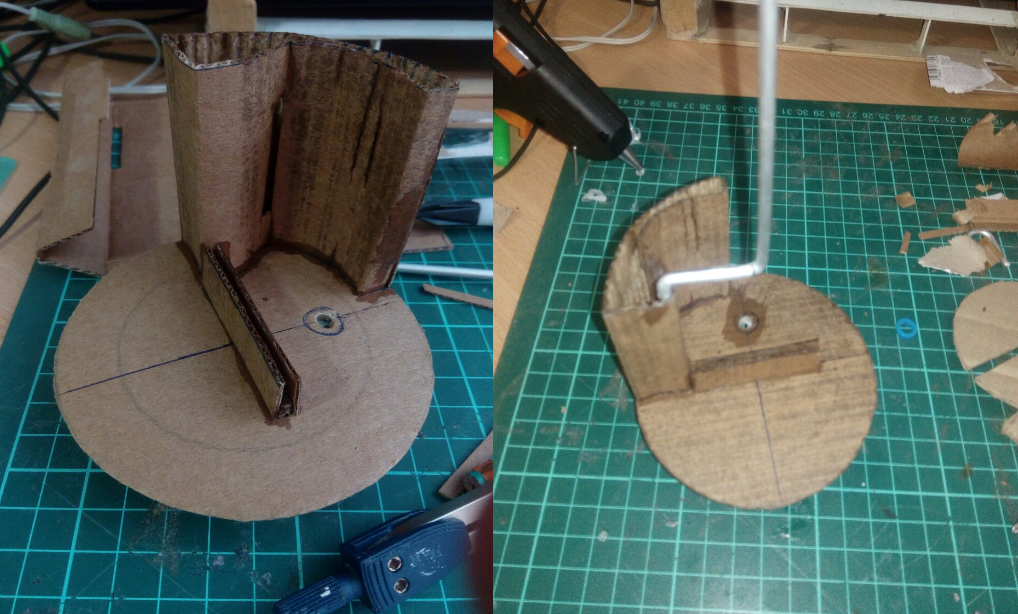
\includegraphics[width = 14cm]{rot.png}
        \caption{Барабан}
        \label{fig: fig1}
    \end{figure}

	\begin{figure}[H]
        \centering
        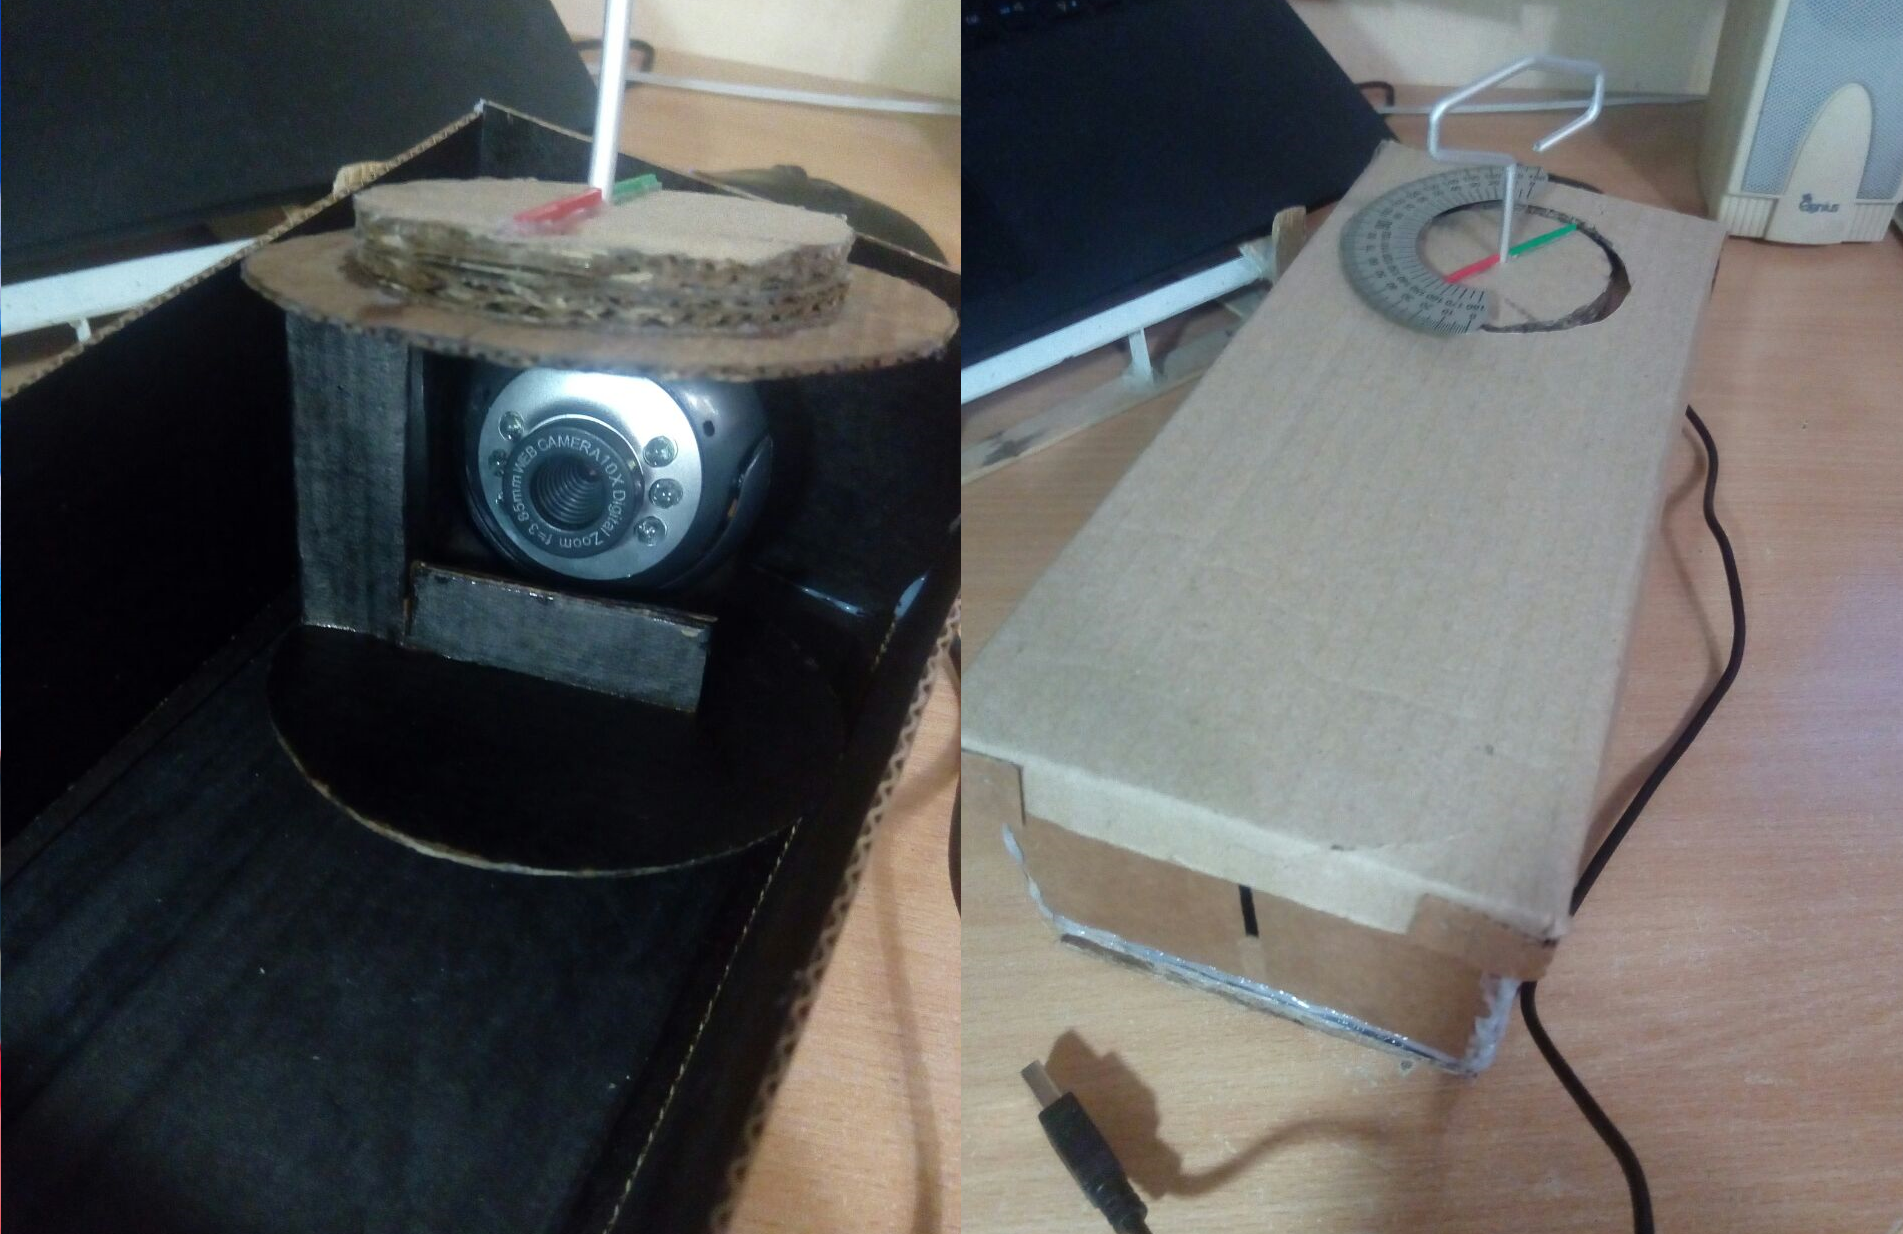
\includegraphics[width = 16cm]{main.png}
        \caption{Собранный спектроскоп}
        \label{fig: fig2}
    \end{figure}

	\subsection{Проведение измерении}
	\subsubsection{Дифракционная решетка 500 штр/мм}

	Первая дифракционная решетка - решетка 500 штр/мм, с периодом d = 0.002 мм. Установим 
	ее в барабан перед камерой. Осветим щели лазером с длиной волны 
	$\lambda = 405 \pm 10 \text{нм}$ и снимим зависимость номера гланого максимума от 
	угла падения пучка света на решетку. 
    Далее везде погрешность $\theta$ возьмем как $\sigma_{\theta} = 5^\circ$, для 
    $sin(\theta)$ погрешность считаем по формуле $cos(\theta)\sigma_{\theta}$

	\begin{table}[!ht]
		\centering
        \caption{Зависимость номера главного максимума от $sin(\theta)$}
		\begin{tabular}{|c|c|c|c|c|c|c|c|c|c|}
		\hline
			m & 0 & 1 & 2 & 3 & 4 & -1 & -2 & -3 & -4 \\ \hline
			$\theta, \circ$ & 0 & 11 & 24 & 39 & 56 & -5 & -21 & -30 & -50 \\ \hline
			$sin(\theta)$ & 0 & 0.19 & 0.41 & 0.63 & 0.83 & -0.09 & -0.36 & -0.50 & -0.77 \\ \hline
		\end{tabular}
		\label{tab: tab1}
	\end{table}

	\begin{multicols}{2}
        \begin{figure*}[ht!]
            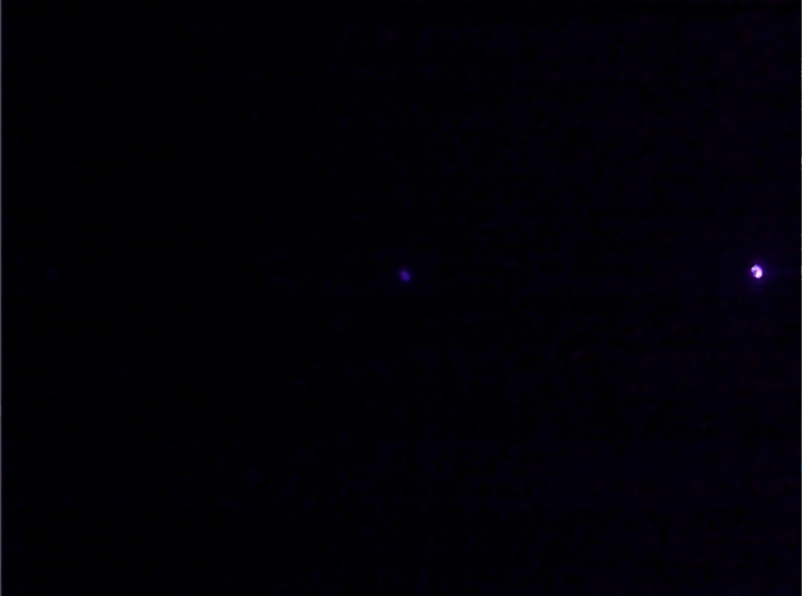
\includegraphics[width=5cm]{500-4.png}\hfill
            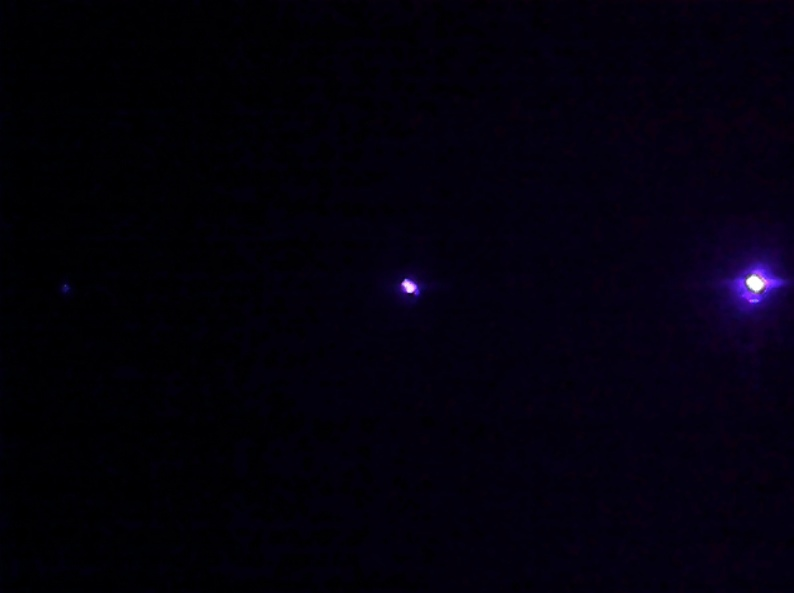
\includegraphics[width=5cm]{500-3.png}\hfill
			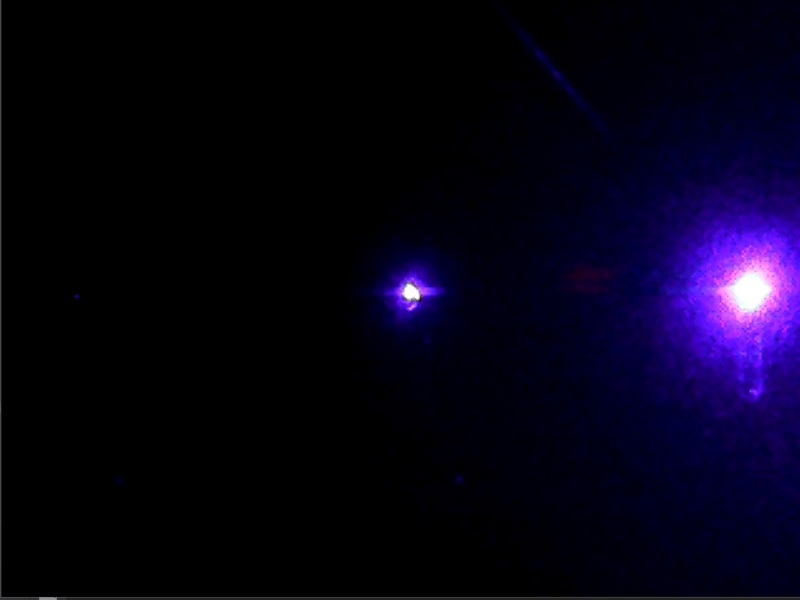
\includegraphics[width=5cm]{500-2.png}\hfill
            \caption{-4, -3 и -2 главные максимумы для решетки в 500 штр/мм}
        \end{figure*}
    \end{multicols}
	\begin{multicols}{2}
        \begin{figure*}[ht!]
            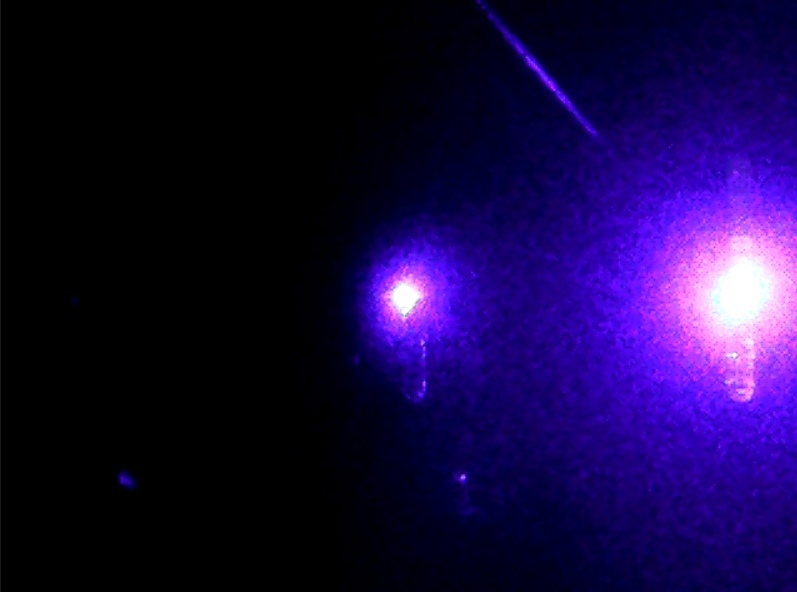
\includegraphics[width=5cm]{500-1.png}\hfill
			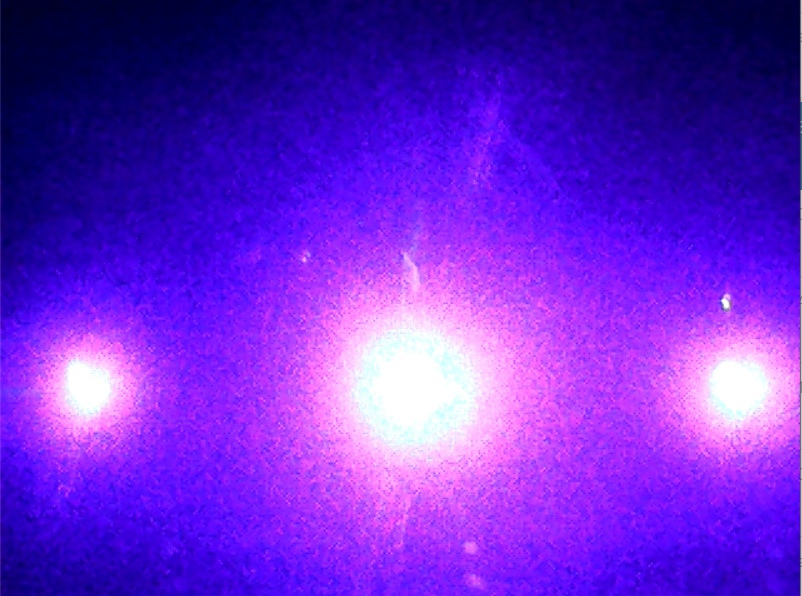
\includegraphics[width=5cm]{500-0.png}\hfill
            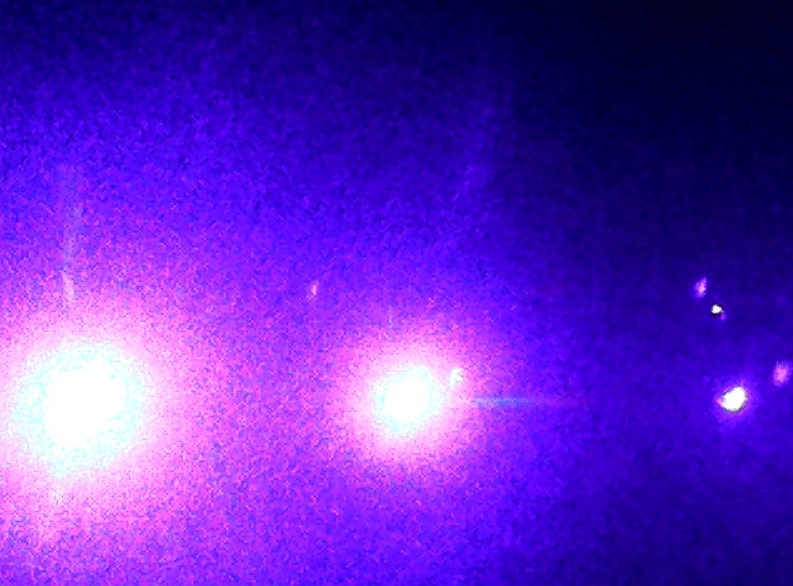
\includegraphics[width=5cm]{500+1.png}\hfill
            \caption{-1, 0 и 1 главные максимумы для решетки в 500 штр/мм}
        \end{figure*}
    \end{multicols}
	\begin{multicols}{2}
        \begin{figure*}[ht!]
			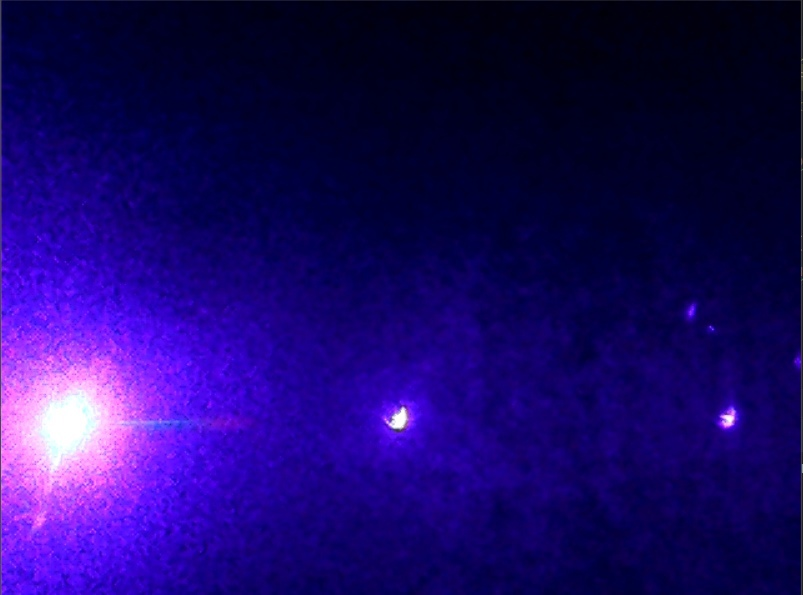
\includegraphics[width=5cm]{500+2.png}\hfill
			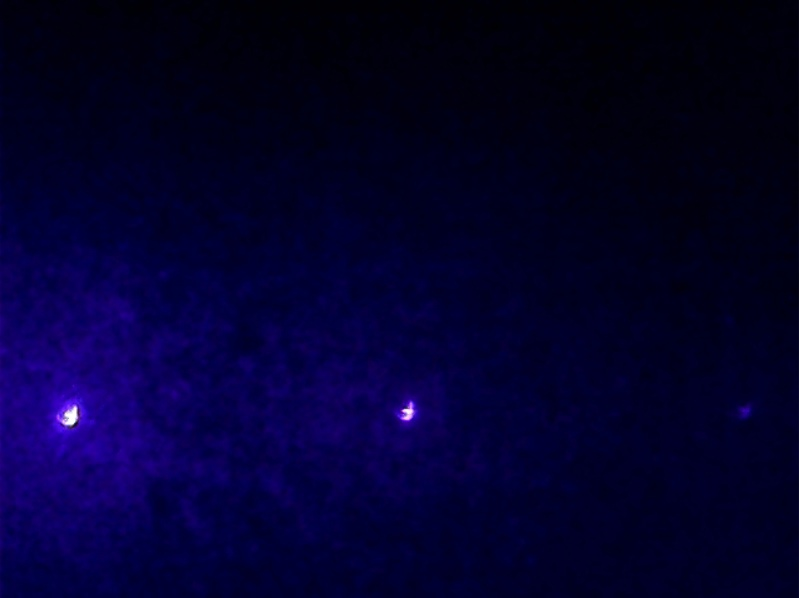
\includegraphics[width=5cm]{500+3.png}\hfill
            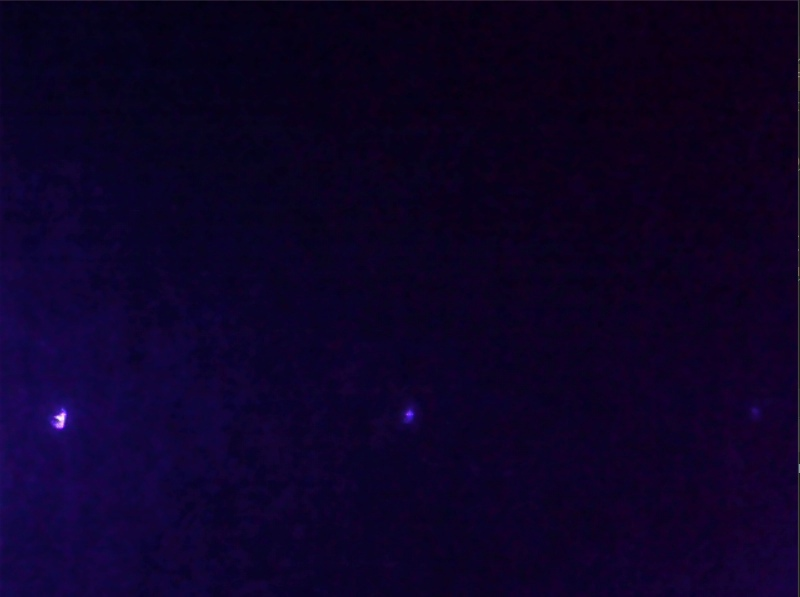
\includegraphics[width=5cm]{500+4.png}\hfill
            \caption{2, 3 и 4 главные максимумы для решетки в 500 штр/мм}
        \end{figure*}
    \end{multicols}

	\begin{figure}[H]
        \centering
        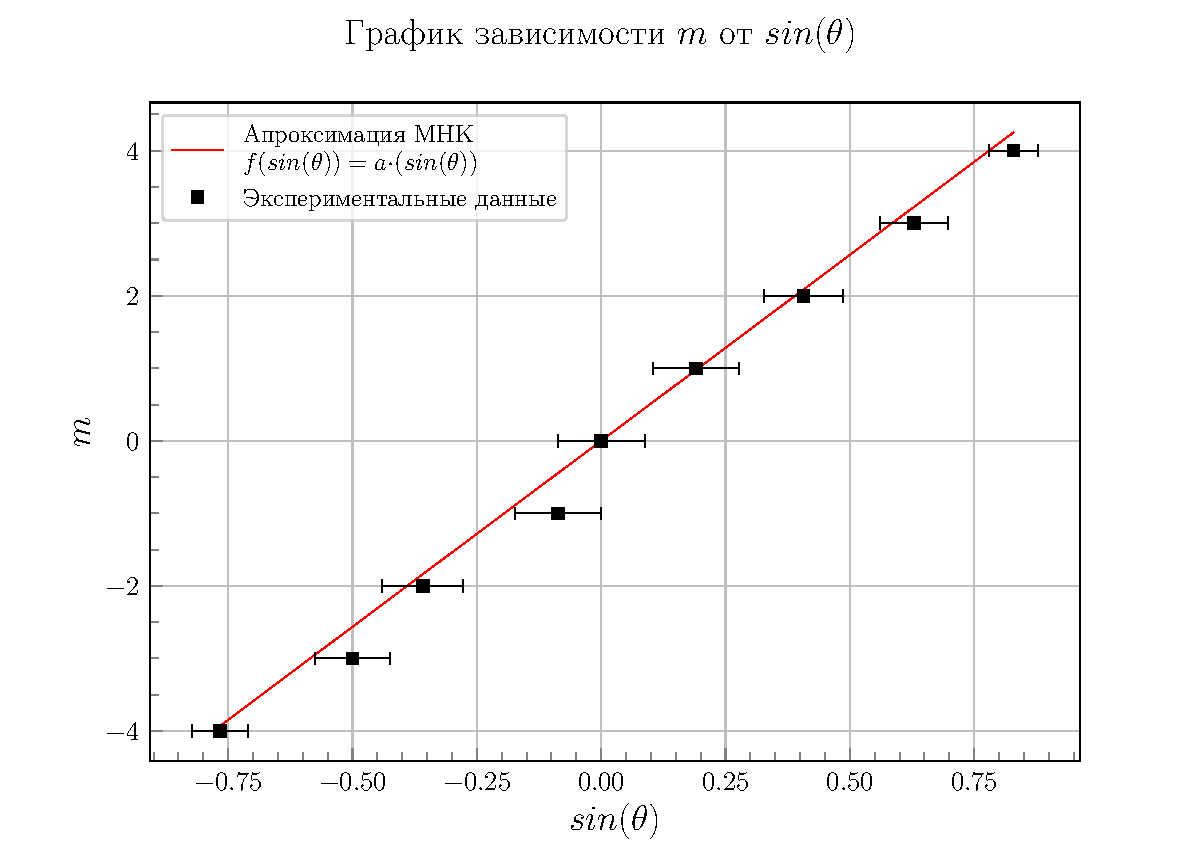
\includegraphics[width = 0.7\textwidth]{500.pdf}
        \label{fig:WT1}
        \caption{График зависимости главного максимума $m$ от синуса угла поворота $sin(\theta)$ для решетки в 500 штр/мм}
    \end{figure}	

	Из МНК получим что угол наклона графика равен $a = 5.1 \pm 0.1$, тогда из формулы 
	максимума дифракционной решетки $m\cdot\lambda = d\cdot sin(\theta)$ получим что 
	$a = \frac{d}{\lambda}$, от сюда $d = a\cdot \lambda = 2.1 \pm 0.1 \text{мкм}$, 
	что сходится с значением указанным на решетке. Погрешность считаем по формуле 
    $\sigma_b = b \sqrt{(\frac{\sigma_a}{a})^2+(\frac{\sigma_{\lambda}}{\lambda})^2}$

	\subsubsection{Дифракционная решетка 1000 штр/мм}

	Вторая дифракционная решетка - решетка 1000 штр/мм, с периодом d = 0.001 мм. Установим 
	ее в барабан перед камерой. Осветим щели лазером с длиной волны 
	$\lambda = 405 \pm 10 \text{нм}$ и снимим зависимость номера гланого максимума от 
	угла падения пучка света на решетку. 

	\begin{table}[!ht]
		\centering
		\caption{Зависимость номера главного максимума от $sin(\theta)$ для решетки 1000 штр/мм}
		\begin{tabular}{|c|c|c|c|c|c|}
		\hline
			m & 0 & 1 & 2 & -1 & -2 \\ \hline
			$\theta, \circ$ & 0 & 24 & 59 & -20 & -50 \\ \hline
			$sin(\theta)$ & 0 & 0.41 & 0.86 & -0.34 & -0.77 \\ \hline
		\end{tabular}
		\label{tab: tab2}
	\end{table}

	\begin{figure}[H]
        \centering
        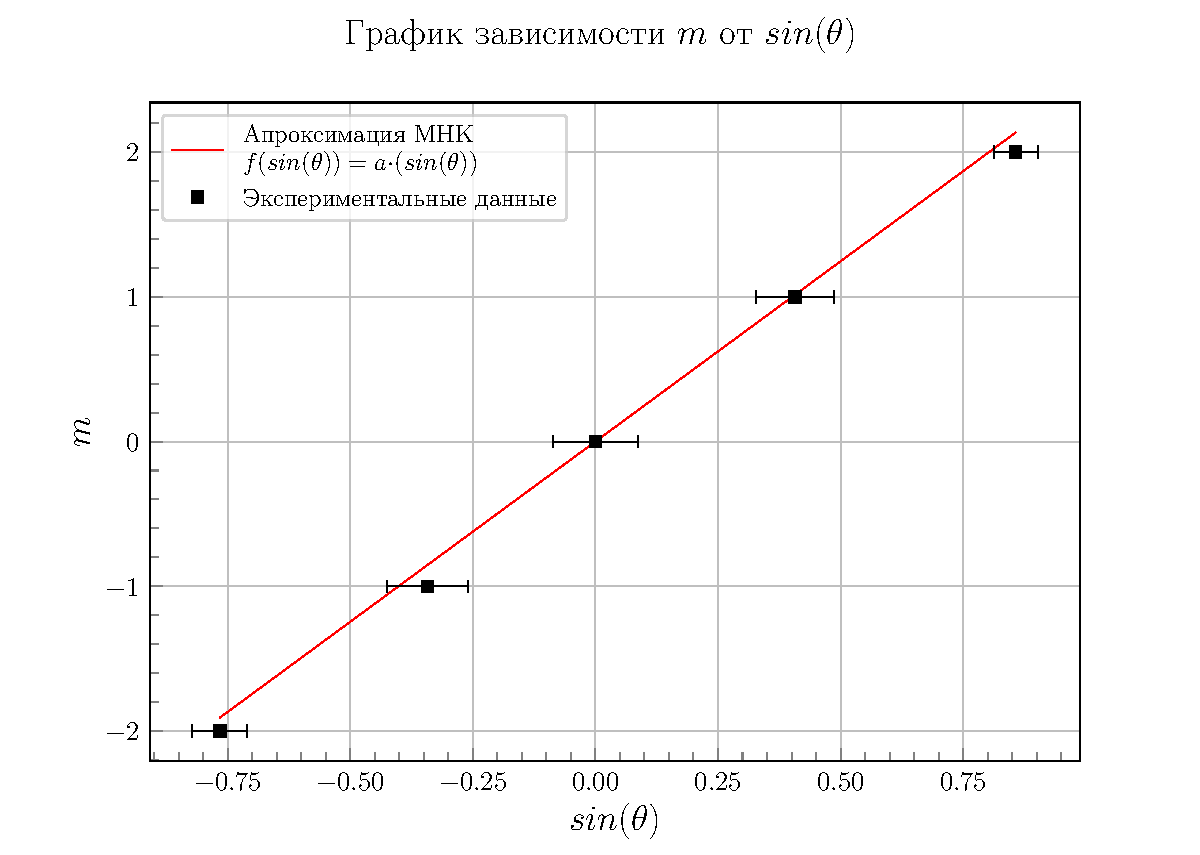
\includegraphics[width = 0.7\textwidth]{1000.pdf}
        \caption{График зависимости главного максимума $m$ от синуса угла поворота $sin(\theta)$  для решетки в 1000 штр/мм}
        \label{fig:WT123}
    \end{figure}	

	\begin{multicols}{2}
        \begin{figure*}[ht!]
            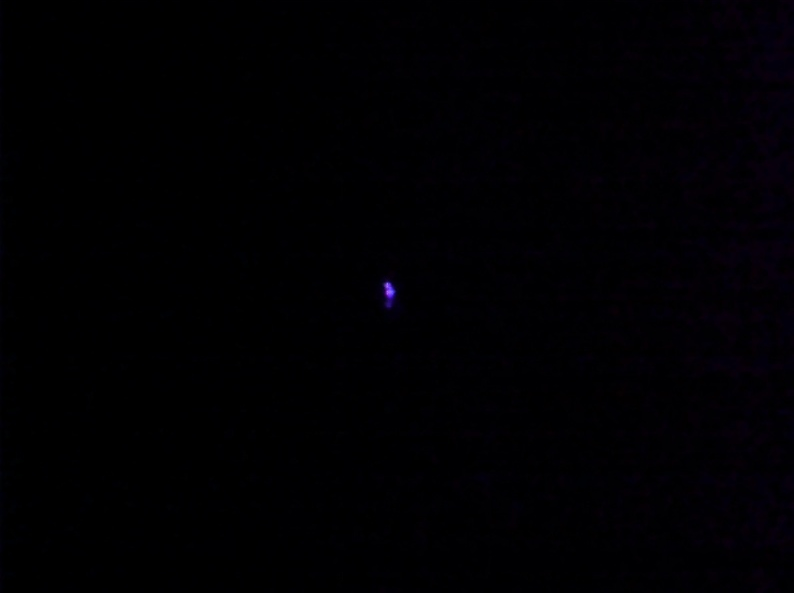
\includegraphics[width=5cm]{1000-2.png}\hfill
            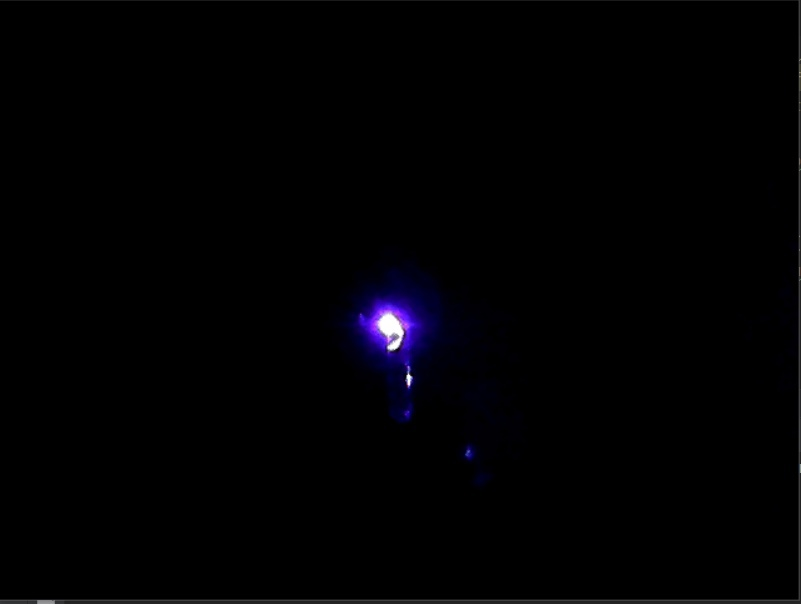
\includegraphics[width=5cm]{1000-1.png}\hfill
			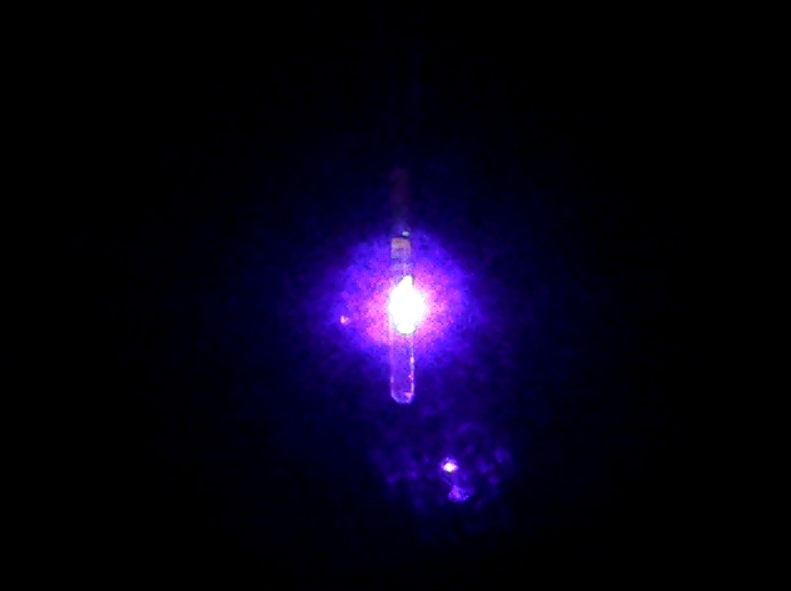
\includegraphics[width=5cm]{1000-0.png}\hfill
            \caption{-2, -1 и 0 главные максимумы для решетки в 1000 штр/мм}
        \end{figure*}
    \end{multicols}
	\begin{multicols}{2}
        \begin{figure*}[ht!]
            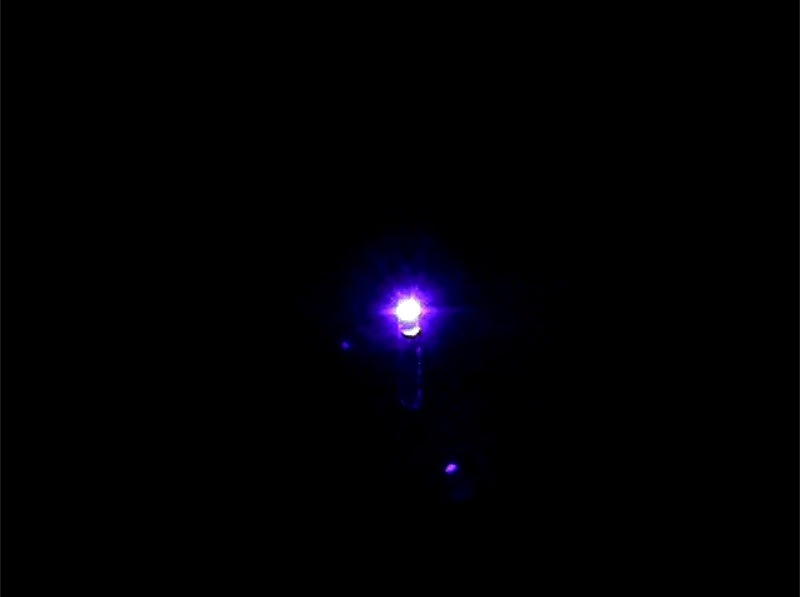
\includegraphics[width=8cm]{1000+1.png}\hfill
			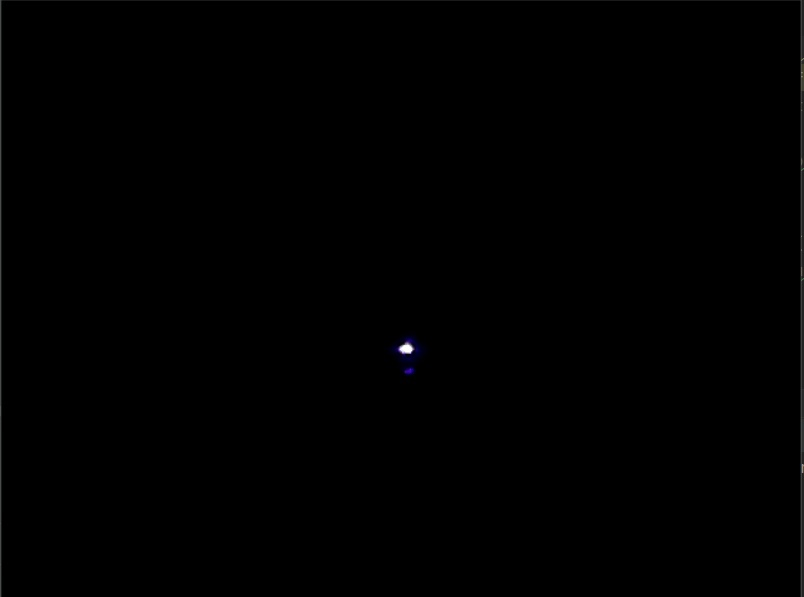
\includegraphics[width=8cm]{1000+2.png}\hfill
            \caption{1 и 2 главные максимумы для решетки в 1000 штр/мм}
        \end{figure*}
    \end{multicols}


    
  

	Из МНК получим что угол наклона графика равен $a = 2.5 \pm 0.1$, тогда из формулы 
	максимума дифракционной решетки $m\cdot\lambda = d\cdot sin(\theta)$ получим что 
	$a = \frac{d}{\lambda}$, от сюда $d = a\cdot \lambda = 1.01 \pm 0.04 \;\text{мкм}$, 
	что сходится с значением указанным на решетке.

	\subsubsection{Двойная дифракционная решетка}

	Третья дифракционная решетка - двойная решетка, с периодами d1 = d2 = 0.0019 мм. 
	Установим ее в барабан перед камерой. Осветим щели лазером с длиной волны 
	$\lambda = 405 \pm 10 \text{нм}$ и снимим зависимость номера гланого максимума от 
	угла падения пучка света на решетку. 

	\begin{table}[!ht]
		\centering
		\caption{Зависимость номера главного максимума от $sin(\theta)$ для двойной решетки}
		\begin{tabular}{|c|c|c|c|c|c|c|c|c|c|c|c|c|}
		\hline
			m & 0 & 1 & 2 & 3 & 4 & 5 & 6 & 7 & -1 & -2 & -3 & -4 \\ \hline
			$\theta, \circ$ & 0 & 6 & 9 & 14 & 18 & 26 & 30 & 37 & -1 & -7 & -9 & -12  \\ \hline
			$sin(\theta)$ & 0 & 0.10 & 0.16 & 0.24 & 0.31 & 0.44 & 0.50 & 0.60 & -0.02 & -0.12 & -0.16 & -0.21 \\ \hline
			m  & -5 & -6 & -7 & ~ &  ~ &  ~ &  ~&  ~ & ~ &  ~&  ~ &  ~ \\ \hline
			$\theta, \circ$ & -19 & -23 & -30 & ~& ~ &  ~ &  ~ &  ~&  ~ & ~ &  ~&  ~ \\ \hline
			$sin(\theta)$  & -0.33 & -0.39 & -0.50 & ~& ~ &  ~ &  ~ &  ~&  ~ & ~ &  ~&  ~ \\ \hline
		\end{tabular}
		\label{tab: tab3}
	\end{table}

	\FloatBarrier


	\begin{multicols}{2}
        \begin{figure*}[!ht]
            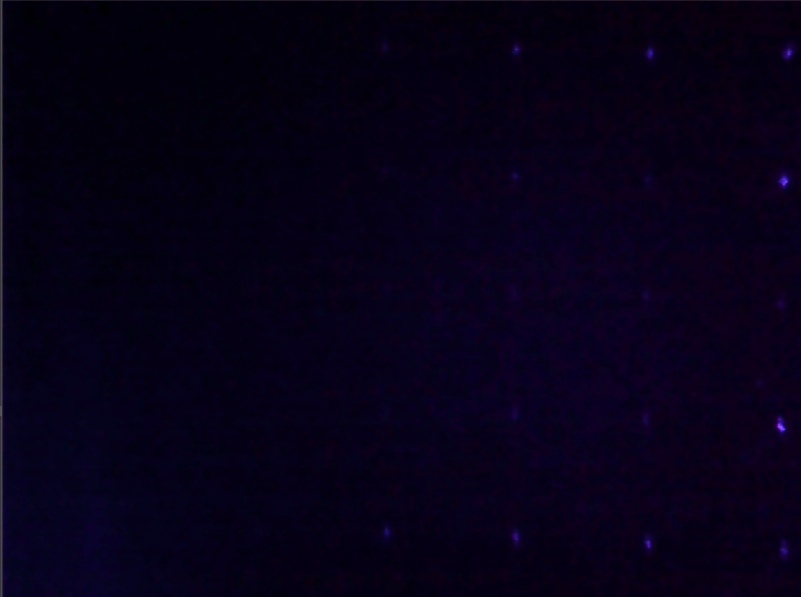
\includegraphics[width=4.5cm]{2-7.png}\hfill
            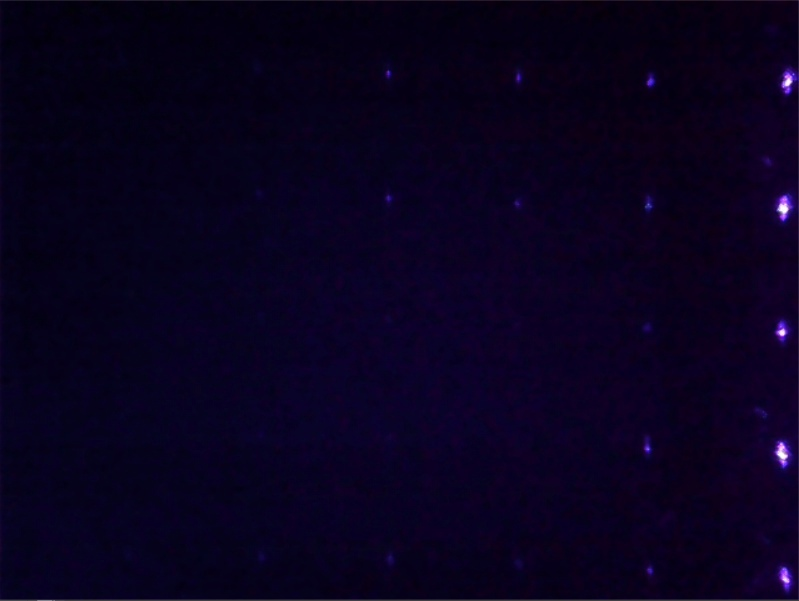
\includegraphics[width=4.5cm]{2-6.png}\hfill
			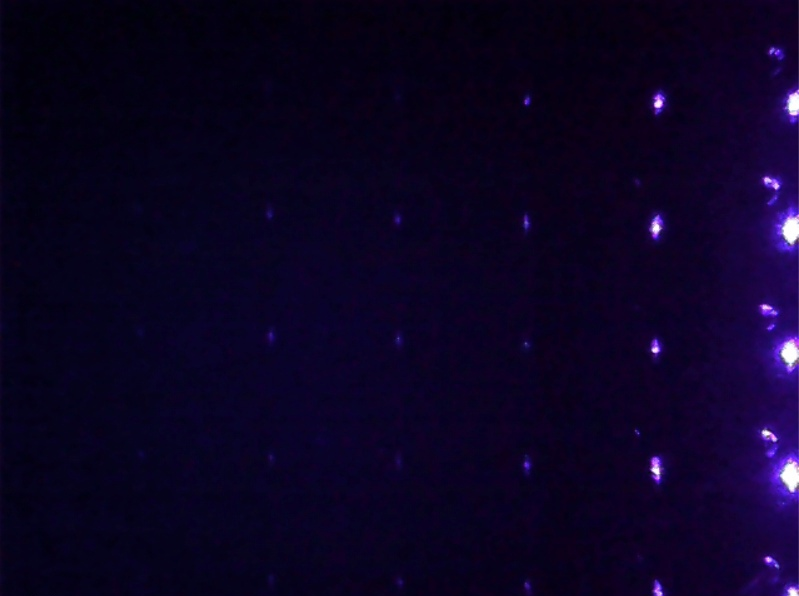
\includegraphics[width=4.5cm]{2-5.png}\hfill
            \caption{-7, -6 и -5 главные максимумы для двойной решетки}
        \end{figure*}
    \end{multicols}
	\begin{multicols}{2}
        \begin{figure*}[!ht]
            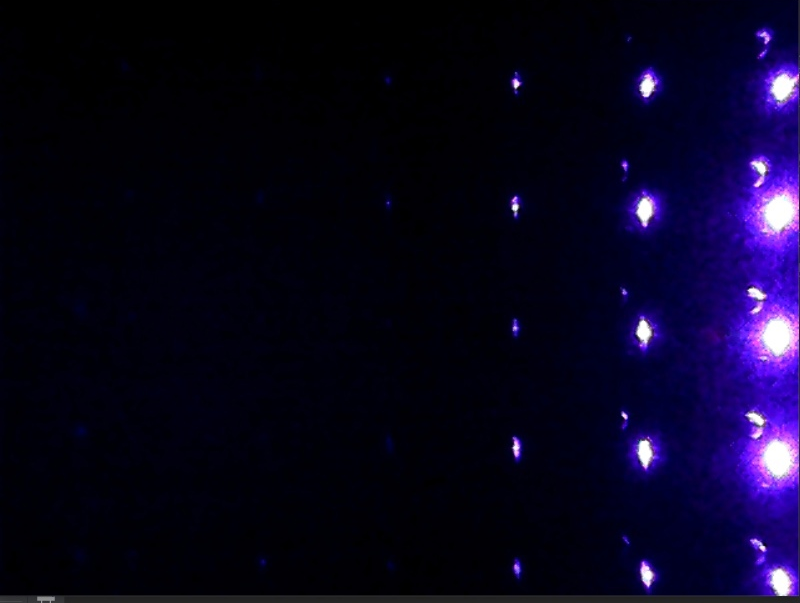
\includegraphics[width=4.5cm]{2-4.png}\hfill
            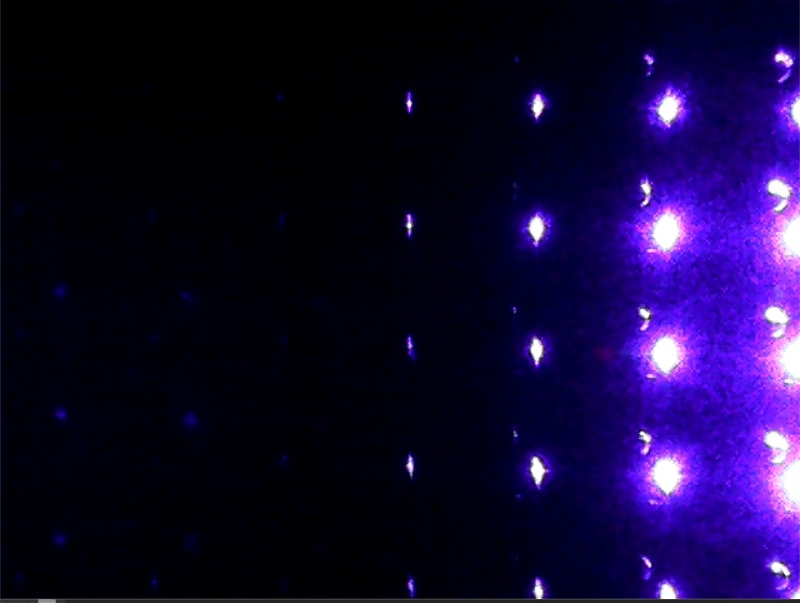
\includegraphics[width=4.5cm]{2-3.png}\hfill
			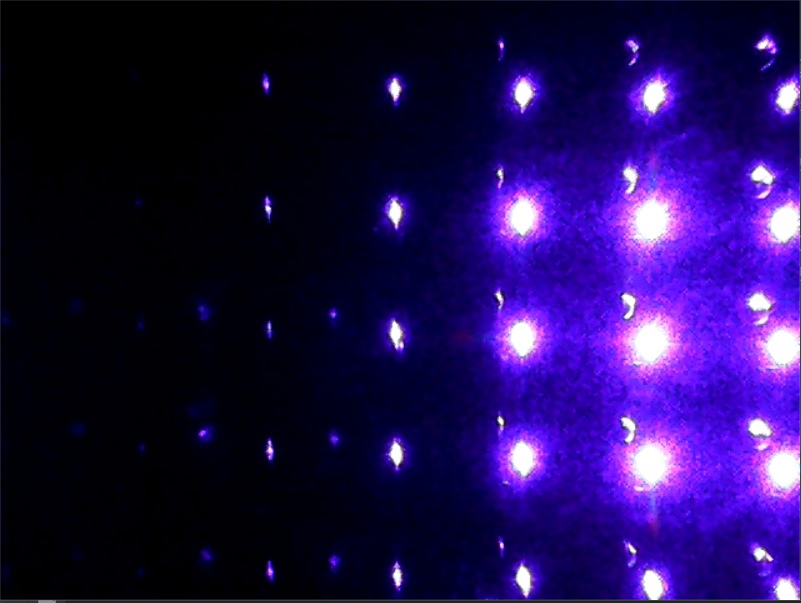
\includegraphics[width=4.5cm]{2-2.png}\hfill
            \caption{-4, -3 и -2 главные максимумы для двойной решетки}
        \end{figure*}
    \end{multicols}
	\begin{multicols}{2}
        \begin{figure*}[!ht]
            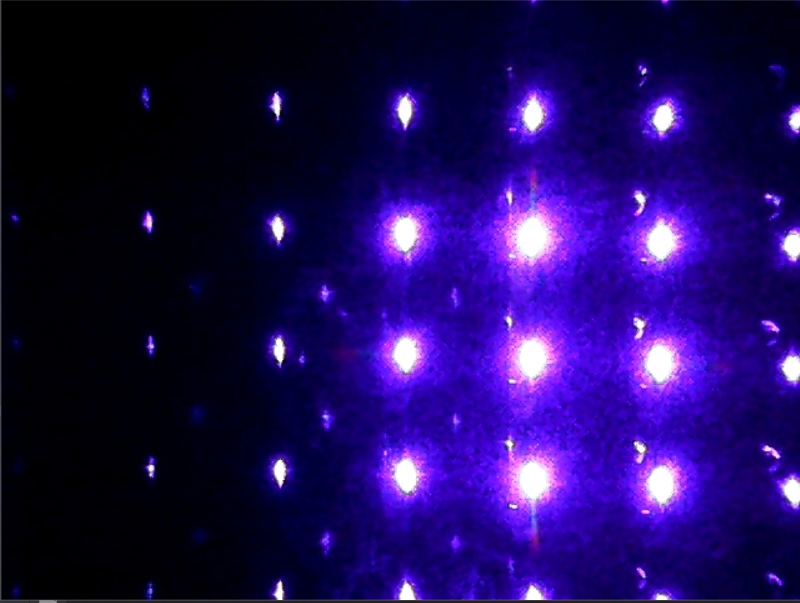
\includegraphics[width=4.5cm]{2-1.png}\hfill
            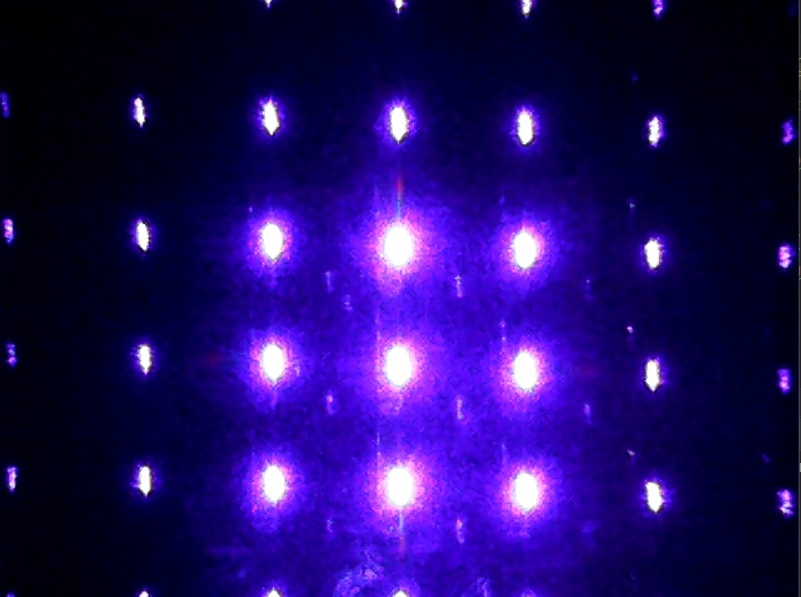
\includegraphics[width=4.5cm]{2-0.png}\hfill
			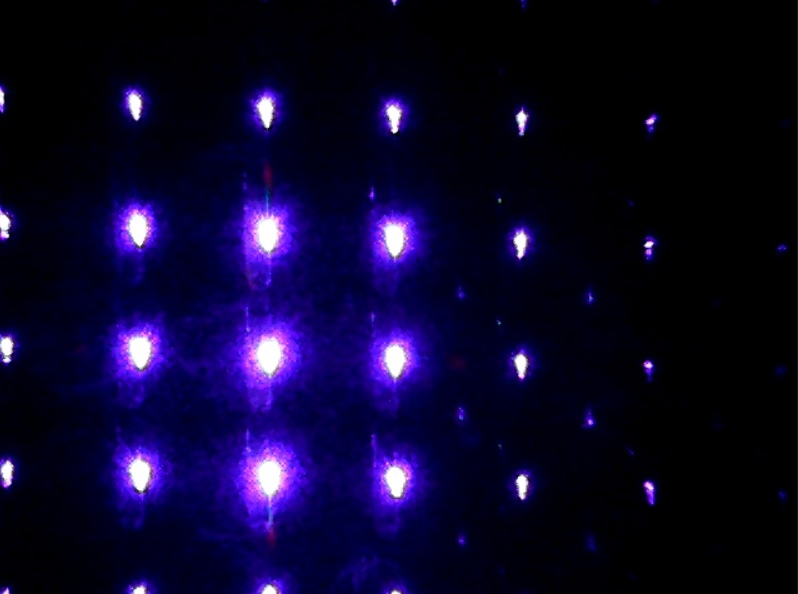
\includegraphics[width=4.5cm]{2+1.png}\hfill
            \caption{-1, 0 и 1 главные максимумы для двойной решетки}
        \end{figure*}
    \end{multicols}
	\begin{multicols}{2}
        \begin{figure*}[!ht]
            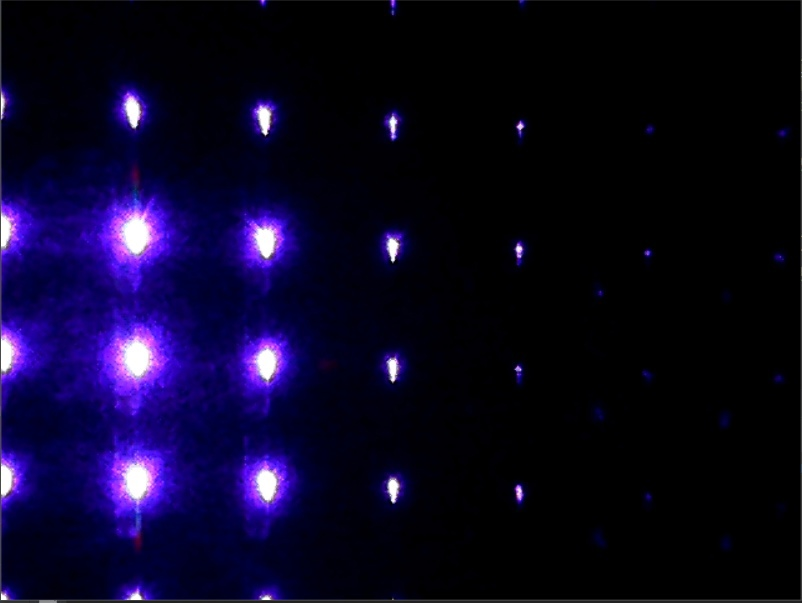
\includegraphics[width=4.5cm]{2+2.png}\hfill
            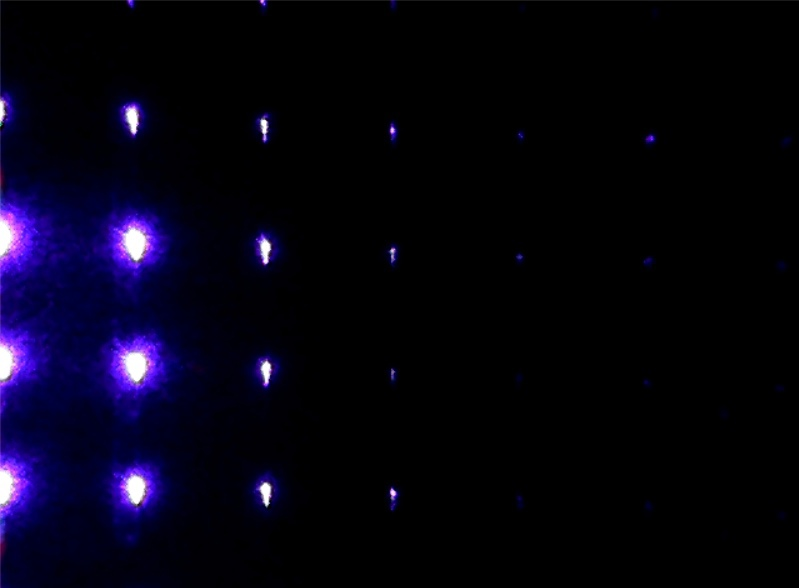
\includegraphics[width=4.5cm]{2+3.png}\hfill
			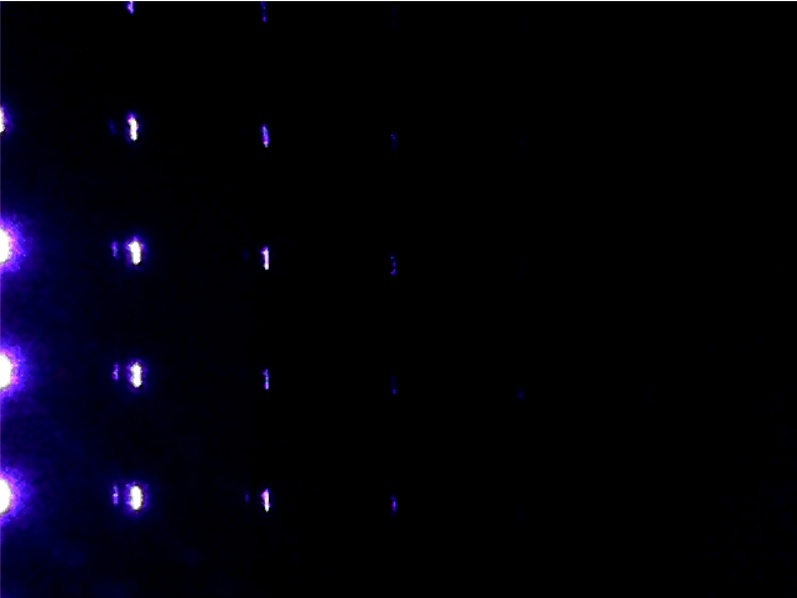
\includegraphics[width=4.5cm]{2+4.png}\hfill
            \caption{2, 3 и 4 главные максимумы для двойной решетки}
        \end{figure*}
    \end{multicols}
	\begin{multicols}{2}
        \begin{figure*}[!ht]
            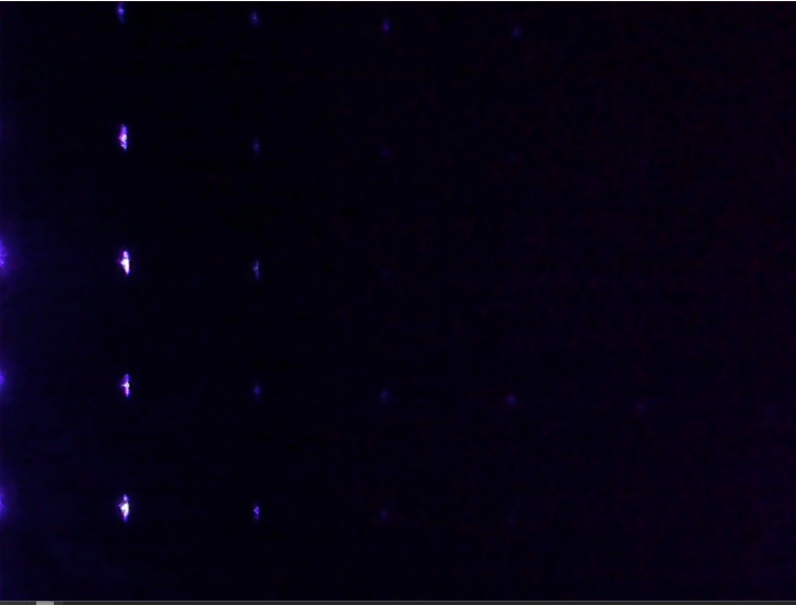
\includegraphics[width=4.5cm]{2+5.png}\hfill
            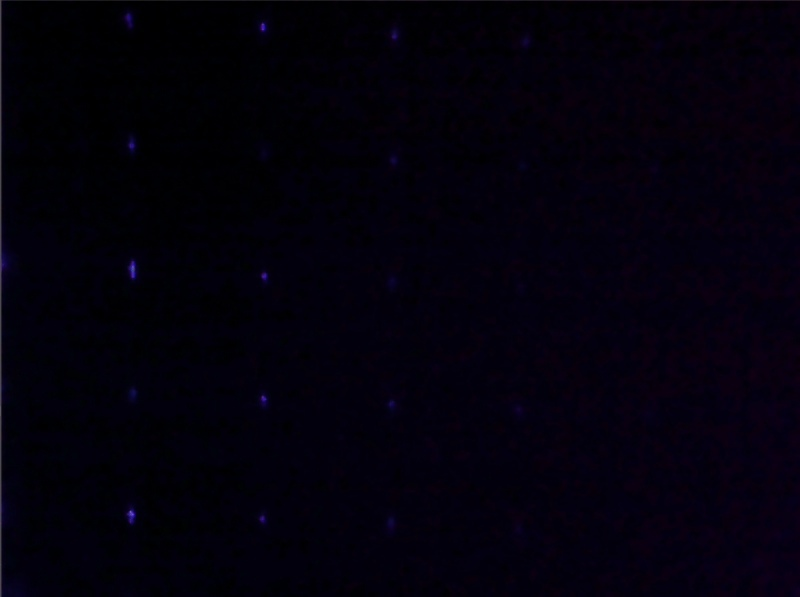
\includegraphics[width=4.5cm]{2+6.png}\hfill
			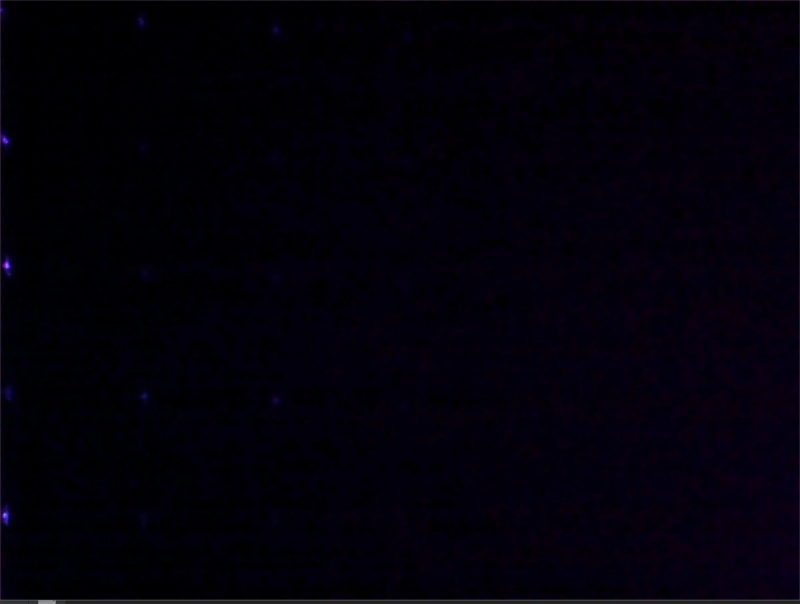
\includegraphics[width=4.5cm]{2+7.png}\hfill
            \caption{5, 6 и 7 главные максимумы для двойной решетки}
        \end{figure*}
    \end{multicols}


	\FloatBarrier

	% \begin{table}[!ht]
	% 	\centering
	% 	\begin{tabular}{|c|c|c|c|}
	% 	\hline
	% 		m  & -5 & -6 & -7 \\ \hline
	% 		$\theta, \circ$ & -19 & -23 & -30 \\ \hline
	% 		$sin(\theta)$  & -0.33 & -0.39 & -0.50 \\ \hline
	% 	\end{tabular}
	% 	\label{tab: tab4}
	% 	\caption{Зависимость номера главного максимума от $sin(\theta)$ для двойной решетки}
	% \end{table}
	

	\begin{figure}[H]
        \centering
        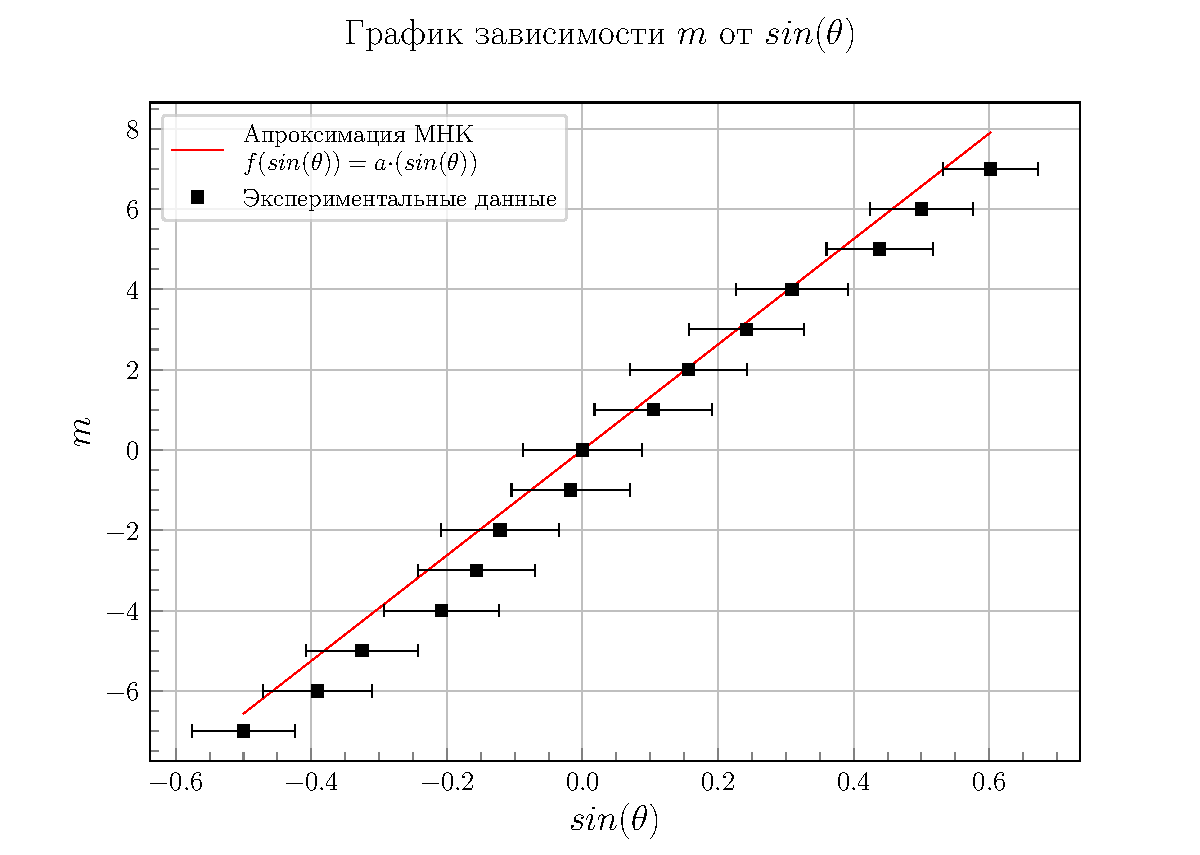
\includegraphics[width = 0.7\textwidth]{2.pdf}
        \caption{График зависимости главного максимума $m$ от синуса угла поворота $sin(\theta)$  для двойной решетки}
        \label{fig:WT1234}
    \end{figure}
	
	
   
	{Из МНК получим что угол наклона графика равен $a = 13.1 \pm 0.5$, тогда из формулы 
	максимума дифракционной решетки $m\cdot\lambda = d\cdot sin(\theta)$ получим что 
	$a = \frac{d}{\lambda}$, от сюда $d = a\cdot \lambda = 5.3 \pm 0.3\;\text{мкм}$, 
	видно что значение не совпадает с тем что написано на решётке. Полученный результат 
	в 2.8 раз превышает тот что написан на решетке.}
	\section{Обсуждение результатов}
	
	В итоге для дифракционной решетки 500 штр/мм получили $d = 2.1 \pm 0.1 \;\text{мкм}$, что совпадает с 
	величиной, указанной на решетке $d = 2 \;\text{мкм}$. Для дифракционной решетки 1000 штр/мм получили 
	$d = 1.01 \pm 0.04 \;\text{мкм}$, что совпадает с величиной, указанной на решетке $d = 1 \;\text{мкм}$. 
	Для двойной дифракционной решетки с $d = 1.9 \;\text{мкм}$ получили $d = 5.3 \pm 0.3 \;\text{мкм}$, что 
	отличается от величины, указанной на самой решетке примерно в 2.8 раз.
	
	Посмотрим на эту дифракционную решетку в микроскоп и сравним с решеткой 500 штр/мм, у которой 
	$d = 2 \;\text{мкм}$, что было подтверждено экспериментально. Из рисунка (\ref{fig:WT12345}) 
	можно увидеть, что действительно период двойной решетки в $2.5-3$ превосходит период от решетки 
	500 штр/мм, то есть равен посчитанному значению. Предполагается, что производитель указал неверную 
	величину на этой решетке.

	
	\newpage

    \begin{figure}[H]
        \centering
        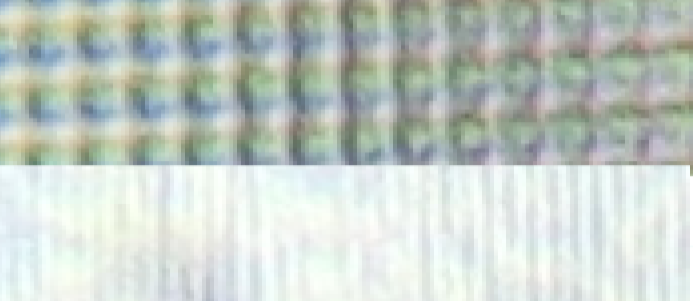
\includegraphics[width = 0.7\textwidth]{micro.png}
        \caption{Решетки под микроскопом, сверху двойная решетка, снизу 500 штр/мм}
        \label{fig:WT12345}
    \end{figure}
	
	\section{Вывод}
	Собрали спектроскоп на основе дифракционной решётки 
	и нашли периоды дифракционных решеток.



 \end{document}